\chapter{Literature review}

\section{Basic aviation terminologies}

\subsection{UAV or Drone}
UAV is short for Unmanned Aerial Vehicle, in other words an airborne vehicle that is capable of movement
without having a pilot on board. Drone is a subset of UAV, a vehicle that is capable of autonomous flight.
Usually UAV and the word Drone are used interchangeably in the literature, and it is used so in this thesis.



\subsection{Body axes used in aviation}
In aviation Euler angles are used to describe the orientation of an aircraft. Euler angles are three angles
that describe the orientation of a rigid body with respect to a fixed coordinate system. These axes are 
referred to as Yaw, Pitch and Roll. Rotation around these axes are Yaw, Pitch 
and Roll angles respectively. All three angles follow the right-hand rule. 

Magnetic north is used as reference for Yaw, so an angle of 0$^\circ$ or 360$^\circ$ means that the vehicle
is heading North, 90$^\circ$ means it's heading East. Yaw is sometimes called Heading.

\begin{figure}[!hb]
    \centering
	$\vcenter{\hbox{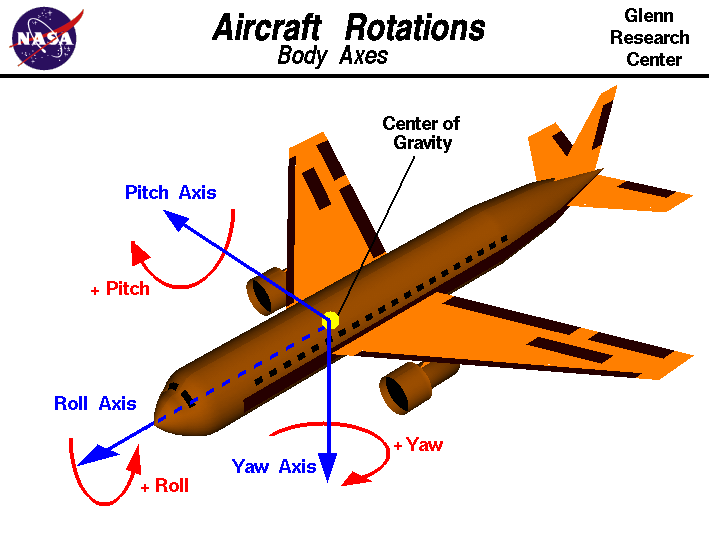
\includegraphics[width=90mm, keepaspectratio]{figures/plane_yaw_pitch_roll.png}}}$
    $\vcenter{\hbox{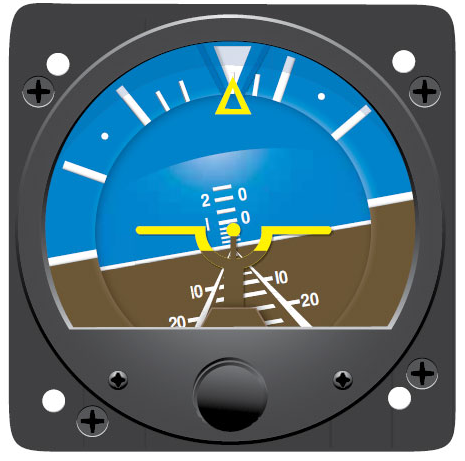
\includegraphics[width=40mm, keepaspectratio]{figures/attitude_indicator.png}}}$
    \caption{Aircraft body axes\cite{AircraftBodyAxes} and attitude instrument}
    \label{fig:aircraft_body_angles}
\end{figure}


Pitch and Roll angles are calculated in reference to the horizontal plane. The normal vector of the horizontal 
plane is used for the calculations, and it is the norm of the gravity vector. It is favorable to use the gravity
vector, because its direction can be measured using an accelerometer. Both Roll and Pitch angles are measured
from -90$^\circ$ to 90$^\circ$. A Pitch of 90$^\circ$ is straight up and 0$^\circ$ is Horizon. If an aircraft
flies with 0$^\circ$ Roll angle, the vehicle is horizontal. On the other hand a 90$^\circ$ Roll angle means
the vehicle is turning right and is perpendicular to the horizon. Pitch is sometimes referred to as Tilt.

The limitation of using Euler angles is reached when Pitch or Roll angles approach 90$^\circ$, because in this 
case one of these angles become parallel with the gravity vector and the other angle cannot be determined, 
due to lack of reference.
Euler angles and singularities are well described in \cite{diebel2006representing}. To avoid singularities
of Euler angles, Unit quaternions can be used. Quaternions are mainly used for calculations, while Euler 
angles are used to provide humanly readable values.

\subsection{Ground Control Station}
A software running on a ground computer, used for receiving in-flight information via telemetry from a UAV.
It displays status and progress of mission, that often includes sensor or video data. It can also be used
for sending commands up to the UAV during flight.

Ground Control Station is often referred to as GCS.

\section{3D LIDAR SLAM Integration with GPS/INS for UAVs in Urban GPS-Degraded Environments}
This paper\cite{hening20173d} presents a data fusion algorithm for estimation of velocity and 
position of a UAV in urban environments where GPS data is partly or completely blocked and is 
unreliable. A LIDAR sensor provides local position updates using SLAM technique, GPS provides 
corrections when available and an Internal Navigation System is used as an additional input to
the Adaptive Extended Kalman filter. The outline of the filter can be seen on figure \ref{fig:haning_filter}

\begin{figure}[!ht]
    \centering
	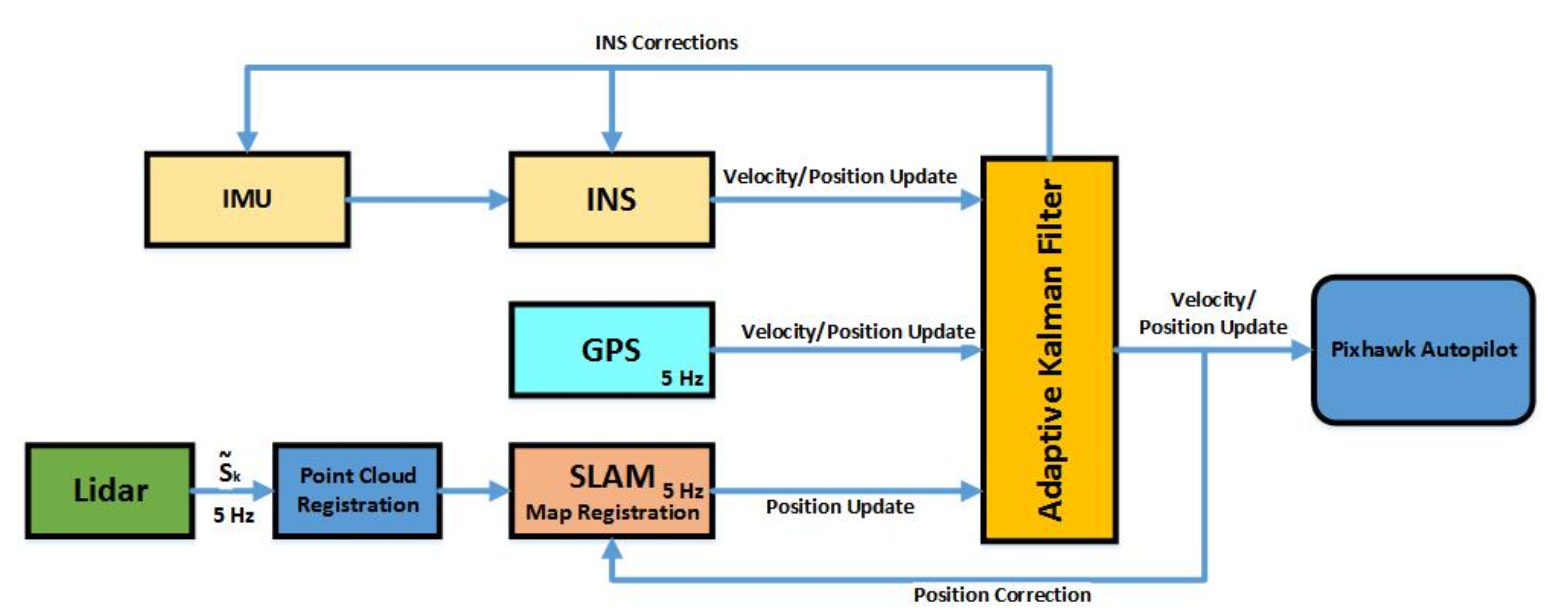
\includegraphics[width=100mm, keepaspectratio]{figures/hening_filter.png}
    \caption{Schematic of LIDAR SLAM, GPS and IMU integration \cite{hening20173d}}
    \label{fig:haning_filter}
\end{figure}

The LIDAR used for measurements is a Velodyne VLP-16, that has a vertical field of view of 30$^\circ$ with a 
vertical resolution of 2$^\circ$. On the horizontal axis it's resolution is 0.1-0.4$^\circ$ and 
rotation rate can be adjusted between 5-20Hz.

The proposed filter is was capable of reducing the GPS drift of 24.3m and LIDAR error of 7.5m to 3.42m.
This shows that fusing GPS, LIDAR and IMU measurements results in a much more accurate position estimate in
GPS-degraded environments. The capabilities of the LIDAR was tested on even an even moon like surface, 
with very few objects that can be detected by the sensor. In this case GPS data is much more accurate, than
LIDAR SLAM results.

\begin{figure}[!ht]
    \centering
	$\vcenter{\hbox{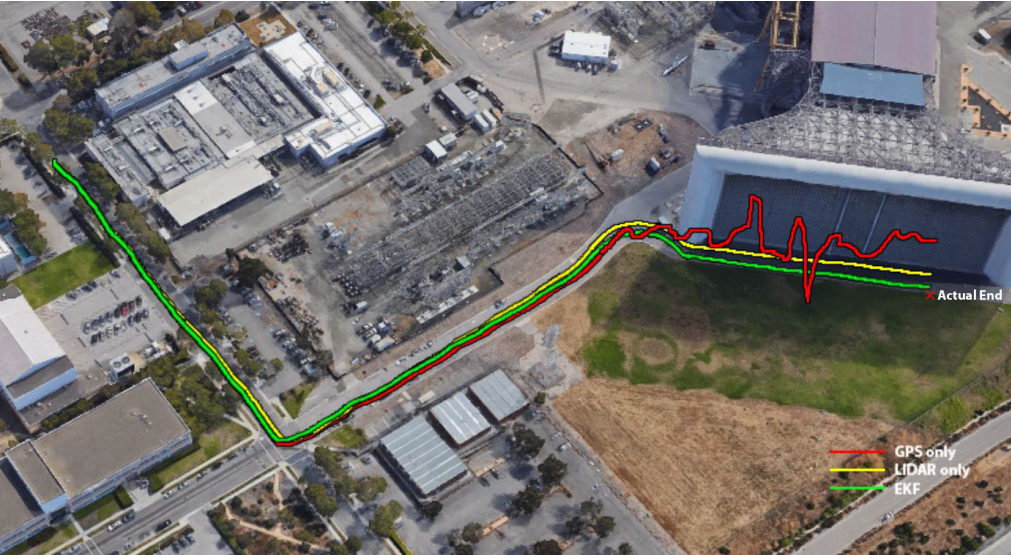
\includegraphics[width=80mm, keepaspectratio]{figures/hening_LIDARvsGPS.png}}}$
	$\vcenter{\hbox{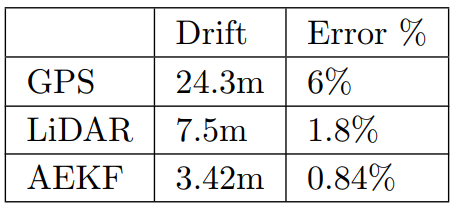
\includegraphics[width=50mm, keepaspectratio]{figures/hening_result.png}}}$
    \caption{GPS, LIDAR and EKF position estimates and position drift after 405 meters\cite{hening20173d}}
    \label{fig:lidar_slam_integration}
\end{figure}




\section{Terabee TeraRanger Tower} \label{TerabeeDescription}
TeraBee offers an off-the-shelf solid-state LIDAR system with the purpose of collision avoidance for drones.
In their solution 8 sensors are evenly distributed around the vertical axis with a controller board in 
the middle. TeraRanger's interface is compatible with Pixhawk 4 flight controller board and 
PX4 flight controller software, that makes integration easy into systems based on these.

\begin{figure}[!ht]
    \centering
    $\vcenter{\hbox{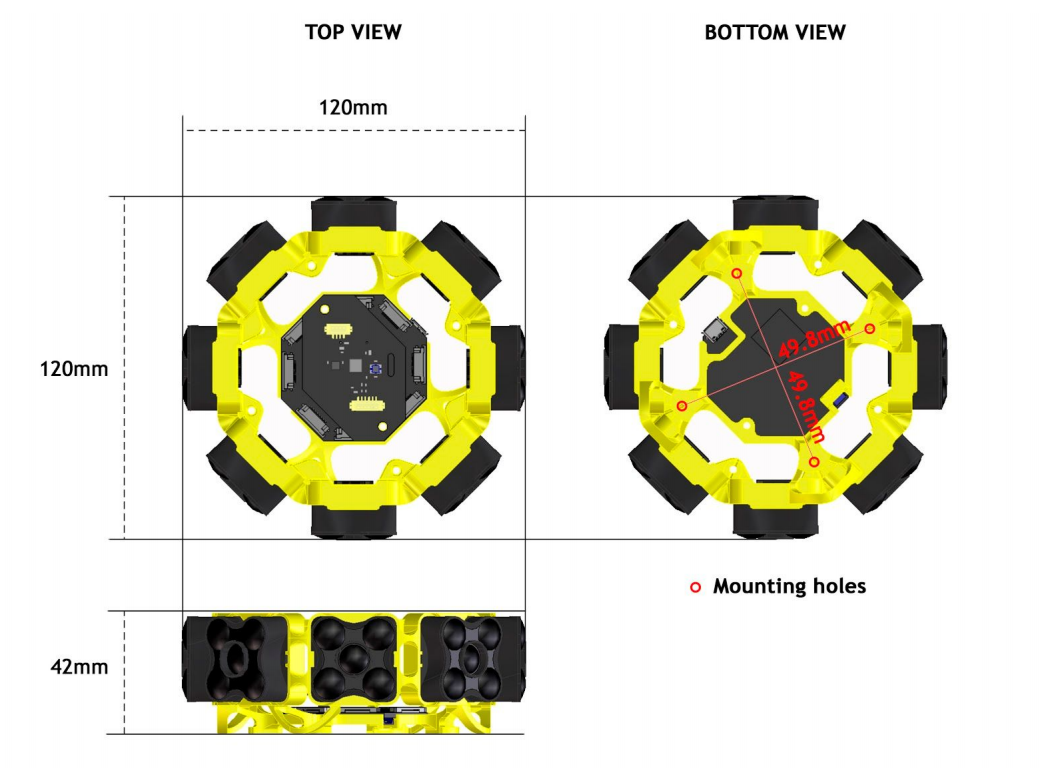
\includegraphics[width=80mm, keepaspectratio]{figures/tera_ranger_tower.png}}}$
    $\vcenter{\hbox{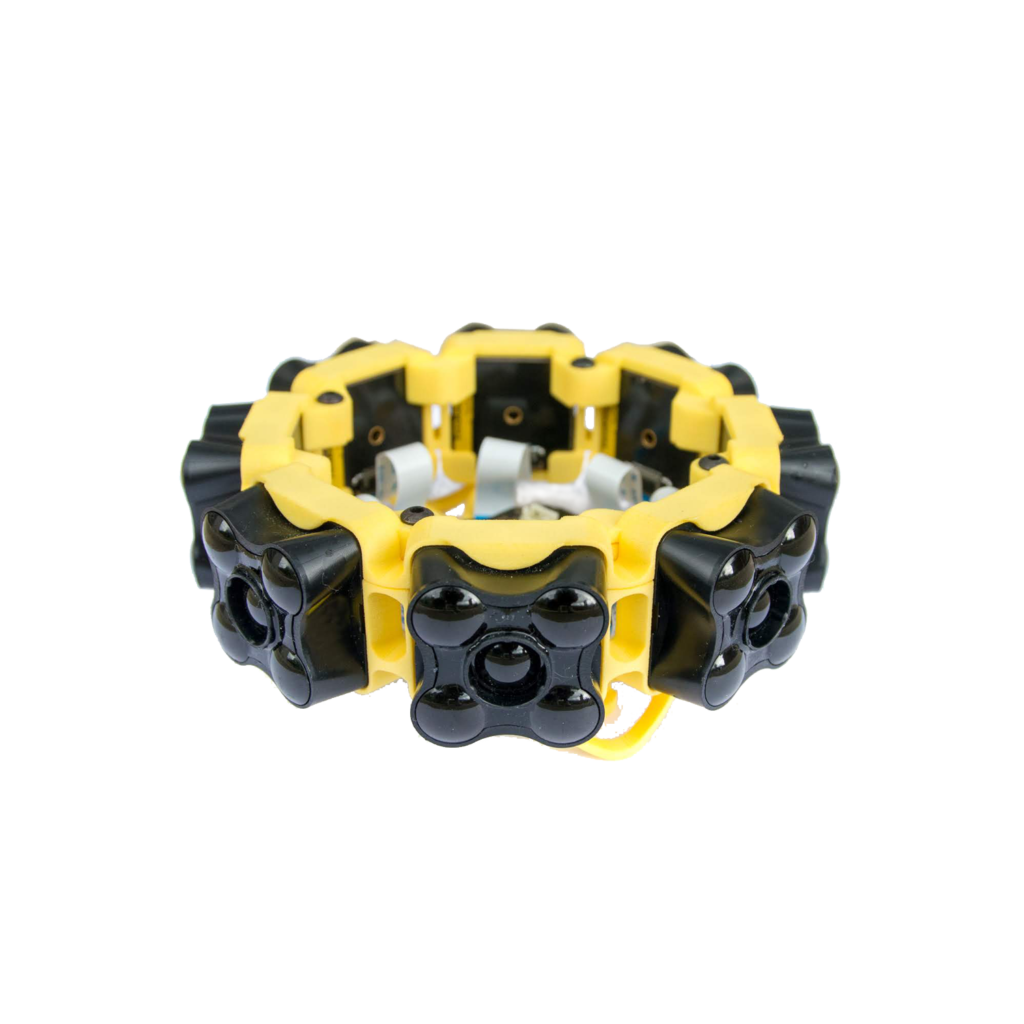
\includegraphics[width=50mm, keepaspectratio]{figures/tera_ranger_tower_2.png}}}$
    \caption{Terabee TeraRanger Tower Evo dimensions}
    \label{fig:teraranger_dimensions}
\end{figure}

Each block of the array is a standalone LIDAR sensor, that can be used separately and supports different
mount configurations. The company offers a long-range and fast-ranging version of these sensors, depending 
on the type an update rate of 320 Hz can be achieved. The fact that system comes with a ROS package and a 
2$^{\circ}$ field of view makes it a potential candidate for indoor mapping and positioning in two dimensions. 
The price of this setup starts from 599 euro\cite{TerabeeTeraRanger}.

\begin{table}[ht]
	\footnotesize
	\centering
	\begin{tabular}{ l c c }
		\toprule
		                & Long-range                                & Fast-ranging \\
		\midrule
		Range           & 0.5m up to 60m                            & 0.75m up to 8m \\
		Update rate     & 120Hz/sensor                              & 320Hz/sensor\\
		Field of View   & 2$^{\circ}$                               & 2$^{\circ}$\\
		Accuracy        & $\pm 4cm$ in the first 14m, 1.5\% above   & $\pm 12cm$\\
		\bottomrule
	\end{tabular}
	\caption{TeraRanger Tower Evo specifications}
	\label{tab:tera_ranger_features}
\end{table}

Terabee provides a tutorial video on their website\cite{TerabeeTeraRanger} how to connect the 
sensor array to a UAV that uses Pixhawk 4 flight controller and the process of configuration 
in two different GCS programs. I have learned that PX4 flight stack supports lidar measurements
for obstacle avoidance and it can be configured from a GCS program. It seems a reasonable choice 
to integrate this feature into such product.

\section{Crazyflie Multi-ranger deck}
The company Bitcraze has developed a mini quadcopter mainly for educational purposes. The current version is
called Crazyflie 2.1 and measures only 92x92mm with a height of 29mm and a weighs 27g.
Extra sensors and peripherals can be attached to the top of the quadcopter using extension boards.

The extension board called Multi-ranger deck has 5 VL53L1X sensors by STMicroelectronics facing forwards, 
backwards, left, right and up. This project is similar to the product of Terabee described in \ref{TerabeeDescription}, 
but in a smaller size factor and with significantly lower weight.

An introduction video can be found on the product website \cite{BitcrazeMultirangerDeck}, where 
a SLAM algorithm is used to create a map and localize the drone. This serves as a proof of concept,
that static VL53L1X sensors can be used for mapping and positioning in two dimensions. The company provided 
no information of the SLAM algorithm used or from the quality of the map.

\begin{figure}[!ht]
    \centering
    $\vcenter{\hbox{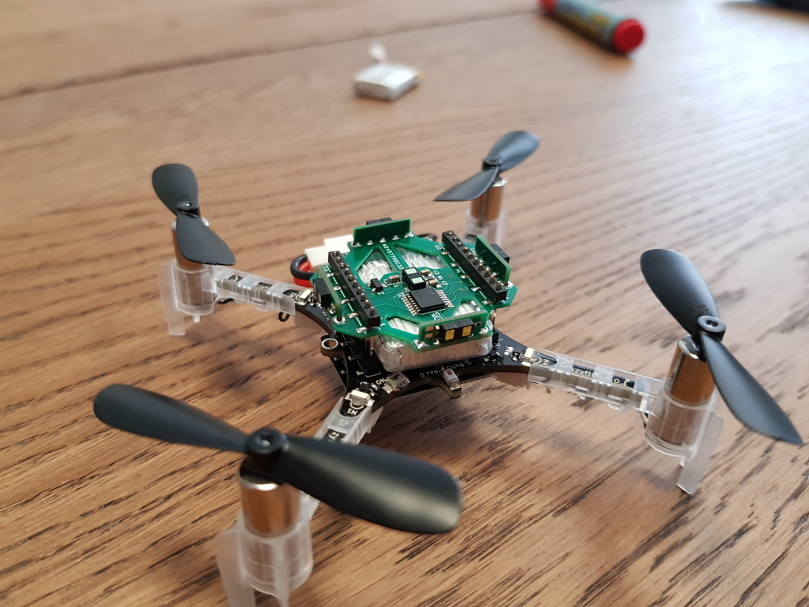
\includegraphics[width=60mm, keepaspectratio]{figures/multiranger_deck.jpg}}}$
    $\vcenter{\hbox{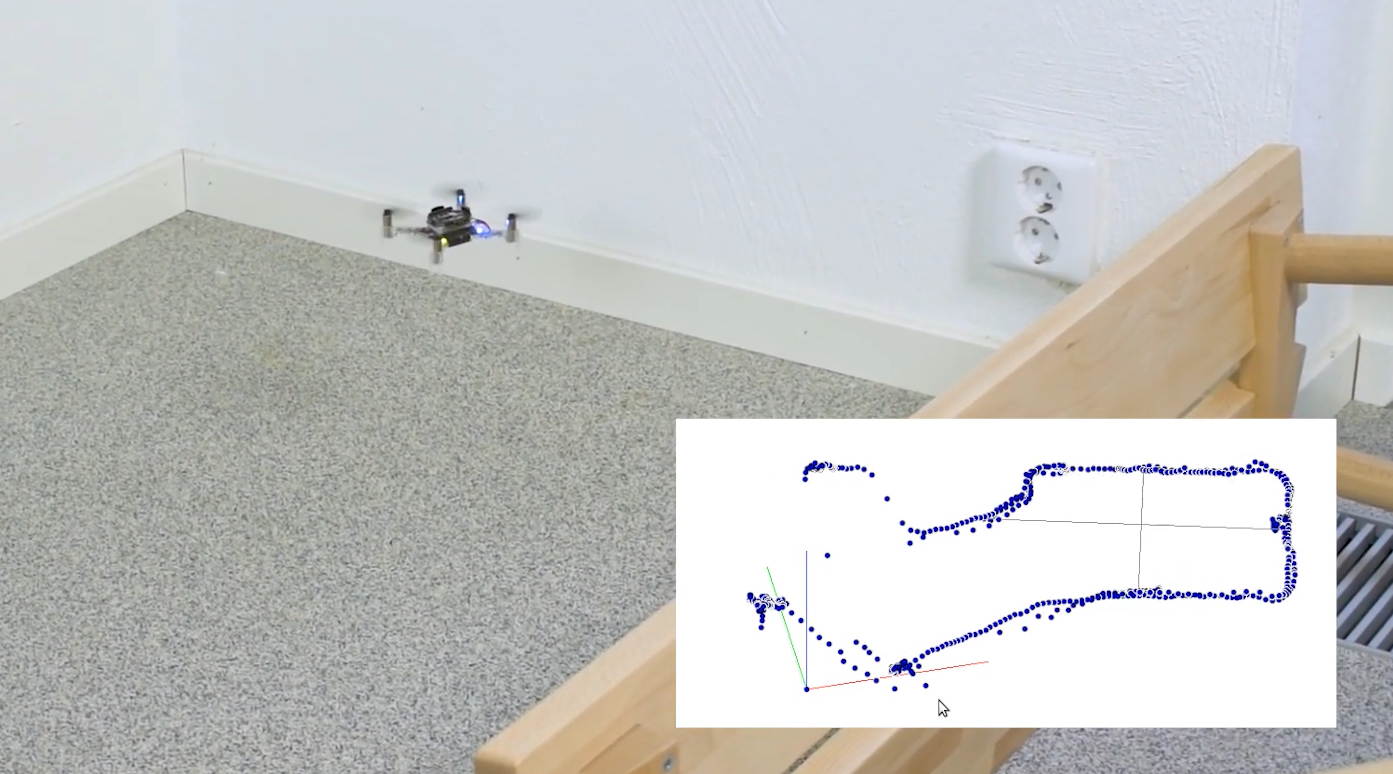
\includegraphics[width=80mm, keepaspectratio]{figures/multiranger_slam.png}}}$
    \caption{Crazyflie Multi-ranger deck, SLAM example project}
    \label{fig:crazyflie_multiranger}
\end{figure}

